%%%%%%%%%%%%%%%%%%%%%%%%%%%%%%%%%%%%%%%%%%%%%%%%%%%%%%%%%
%%             东南大学数电实验报告 LaTeX 模板
%%                SEU-Circuit-Report.cls
%% https://github.com/Teddy-van-Jerry/SEU_Digital_Report
%% ======================================================
%% 版本信息:
%% v1.0 (Nov. 07, 2021)
%% ------------------------------------------------------
%% 模板制作:
%% Teddy van Jerry, (me@teddy-van-jerry.org)
%% * GitHub: https://github.com/Teddy-van-Jerry
%% * Website: https://teddy-van-jerry.org
%% * Blog: https://blog.teddy-van-jerry.org
%% ------------------------------------------------------
%% 使用说明:
%% 1. 编译使用 XeLaTeX 和 Biber
%% 2. 报告基本信息通过修改导言区以 exp 开头的命令
%% 3. 参考文献位于 ref/ref.bib
%% 4. 报告模板依据 MIT License 开源共享
%% ------------------------------------------------------
%% Copyright 2021 (c) Teddy van Jerry
%%
%% Permission is hereby granted, free of charge, to any
%% person obtaining a copy of this software and
%% associated documentation files (the "Software"), to
%% deal in the Software without restriction, including
%% without limitation the rights to use, copy, modify,
%% merge, publish, distribute, sublicense, and/or sell
%% copies of the Software, and to permit persons to whom
%% the Software is furnished to do so, subject to the
%% following conditions:
%%
%% The above copyright notice and this permission notice
%% shall be included in all copies or substantial
%% portions of the Software.
%% 
%% THE SOFTWARE IS PROVIDED "AS IS", WITHOUT WARRANTY OF
%% ANY KIND, EXPRESS OR IMPLIED, INCLUDING BUT NOT
%% LIMITED TO THE WARRANTIES OF MERCHANTABILITY, FITNESS
%% FOR A PARTICULAR PURPOSE AND NONINFRINGEMENT. IN NO
%% EVENT SHALL THE AUTHORS OR COPYRIGHT HOLDERS BE LIABLE
%% FOR ANY CLAIM, DAMAGES OR OTHER LIABILITY, WHETHER IN
%% AN ACTION OF CONTRACT, TORT OR OTHERWISE, ARISING
%% FROM, OUT OF OR IN CONNECTION WITH THE SOFTWARE OR THE
%% USE OR OTHER DEALINGS IN THE SOFTWARE.
%%%%%%%%%%%%%%%%%%%%%%%%%%%%%%%%%%%%%%%%%%%%%%%%%%%%%%%%%%

%% 使用实验报告模板类(字体大小 11pt 约为五号字)
\documentclass[11pt]{SEU-Digital-Report}

%%%%%%%%%%%%%%%%%%%% 报告基本信息 %%%%%%%%%%%%%%%%%%%%
\expno{二} % 实验序号
\expname{基本算术和逻辑运算} % 实验名称
\expauthor{薛宇飞 } % 姓名
\expID{04020235} % 学号
\expmates{} % 同组
\expmatesID{} % 学号(同组)
\expmajor{信息工程} % 专业
\explab{金智楼硬件实验室} % 实验室
\expdate{\today} % 实验日期
\expreportdate{\today} % 实验日期
\expgrade{} % 成绩评定
\exptutor{裴文江} % 评阅教师
%%%%%%%%%%%%%%%%%%%%%%%%%%%%%%%%%%%%%%%%%%%%%%%%%%%%
% \usepackage{xeCJK}
\usepackage{threeparttable} %table添加注释
\usepackage{colortbl}
\newcommand{\grayrow}{\rowcolor[rgb]{ .906, .902, .902}}
\usepackage{pgfplots}
\pgfplotsset{compat=1.11}

%% 报告正文
\begin{document}

% 打印封面页
\exptitlepage

\tableofcontents
\newpage

\section{实验目的与内容}       
\begin{enumerate}
    \item 熟悉算术和逻辑运算指令的功能;
    \item 结合实验教材 \cite{book,guide},进一步了解标志寄存器各标志位的意义和指令执行对它的影响。   
\end{enumerate}

\section{实验任务}
实验全部资料及完整代码详见薛宇飞的 \texttt{GitHub} 主页 \cite{mygit}。

\subsection{运行并检查标志位}
采用单步执行方式执行下列各程序段,检查各标志位的情况。
\begin{lstlisting}[language={[x86masm]Assembler},title=code1]
    MOV AX,0A0A0H
    ADD AX,0FFFFH
    MOV CX,0FF00H  
    ADD AX,CX
    SUB AX,AX
    INC AX
    OR CX,00FFH
    AND CX,0FOFH
    MOV [0010],CX
\end{lstlisting}

\begin{analyze}{指令对标志位的影响}{}

\end{analyze}

\begin{lstlisting}[language={[x86masm]Assembler},title=code2]
    MOV BL,25H
    MOV [0010],04H
    MOV AL,[0010]
    MUL BL
\end{lstlisting}

\begin{analyze}{指令对标志位的影响}{}

\end{analyze}

\begin{lstlisting}[language={[x86masm]Assembler},title=code3]
    MOV BL,04H
    MOV WORD  PTR[0010],0080H
    MOV AX,[0010]
    DIV BL
\end{lstlisting}

\begin{analyze}{指令对标志位的影响}{}

\end{analyze}

\begin{lstlisting}[language={[x86masm]Assembler},title=code4]
    MOV AX,00
    DEC AX
    ADC AX,3FFFH
    ADD AX,AX
    NOT AX
    SUB AX,3
    OR AX,0FBFDH
    AND AX,0AFCFH
    SHL AX,l
    RCL AX,1   
\end{lstlisting}

\begin{analyze}{指令对标志位的影响}{}

\end{analyze}

\subsection{求和与作积}
将寄存器\texttt{BX}作地址指针,自\texttt{BX}所指的内存单元\texttt{(0010H)}开始连续存放着三个无符号数\texttt{(10H、04H、30H)}。试编写程序分别求它们的和与积,并将结果存放在这三个数之后的单元中。
\begin{lstlisting}[language={[x86masm]Assembler},title=code]

\end{lstlisting}

实验结果见图 \ref{fig:rlt2}
\begin{figure}[htbp]
    \centering
    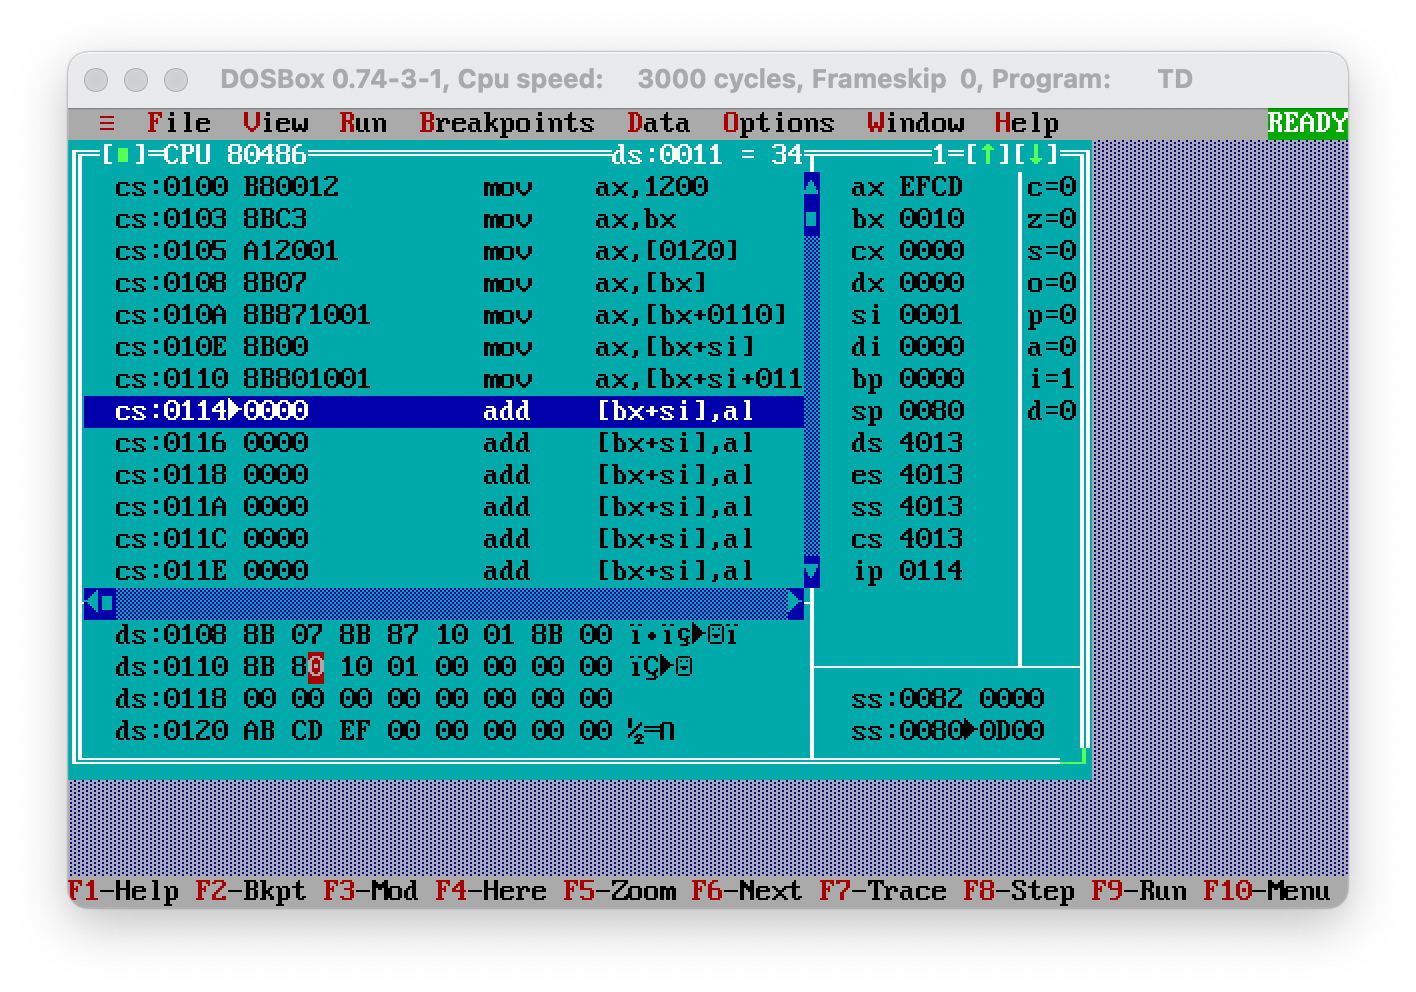
\includegraphics[width=0.7\textwidth]{fig/task4.png}
    \caption{实验二结果}
    \label{fig:rlt2} 
\end{figure}

\subsection{编写功能程序段1}
\begin{enumerate}
    \item 传送\texttt{15H}到\texttt{AL}寄存器;
    \item 将\texttt{AL}的内容乘以2;
    \item 传送\texttt{15H}到\texttt{BL}寄存器;
    \item \texttt{AL}的内容乘以\texttt{BL}的内容。
    \item 求出最后结果\texttt{AX}。
\end{enumerate}

\begin{lstlisting}[language={[x86masm]Assembler},title=code]

\end{lstlisting}

\subsection{编写功能程序段2}
\begin{enumerate}
    \item 从地址\texttt{DS:0000H}单元中,传送一个数据\texttt{58H}到\texttt{AL}寄存器;
    \item 把\texttt{AL}寄存器的内容右移两位;
    \item 再把\texttt{AL}寄存器的内容与字节单元\texttt{DS:0001H}中的数据\texttt{12H}相乘;
    \item 将乘积存入字单元\texttt{DS:0002H}中。
\end{enumerate}

\begin{lstlisting}[language={[x86masm]Assembler},title=code]

\end{lstlisting}

\subsection{清除程序段}
假设下面的程序段用来清除数据段中相应字存储单元的内容(即零送到这些存储单元中去),其偏移地址从\texttt{0010H}到\texttt{001FH}。
\begin{lstlisting}[language={[x86masm]Assembler},title=code]
          MOV SI,0010H
    NEXT: MOV WORD PTR [SI],00
          ADD SI,2
          CMP SI,_____   
          JNE NEXT
\end{lstlisting}

假设要清除偏移地址从\texttt{001FH}到\texttt{0010H}字存储单元中的内容(即由高地址到低地址清零),试编写程序段。
\begin{lstlisting}[language={[x86masm]Assembler},title=code]

\end{lstlisting}

\subsection{尝试\texttt{BCD}码调整指令}
\subsubsection{\texttt{BCD}码任务1}
假设数据段:\texttt{[0000H]=18H, [0001H]=34H, [0010H]=98H, [0011H]=27H} \ref{task6.1}。
\begin{table}[htbp]
    \centering
    \caption{任务表格\label{tab:task6.1}}
    \bgroup\def\arraystretch{1.5}
    \setlength{\tabcolsep}{4.5mm}
        \begin{tabular}{l|c|c}
          \toprule
          \textbf{指令} & \textbf{分析} & \texttt{AL}\\
          \midrule\midrule
          \grayrow  \texttt{MOV AL,[0000H]} & & -\\
                    \texttt{ADD AL,[0010H]} & & \\
          \grayrow  \texttt{DAA} & & \\
                    \texttt{MOV [0020H],AL}& & -\\
          \grayrow  \texttt{MOV AL,[0001H]} & & -\\
                    \texttt{ADC AL,[0011H]} & & \\
          \grayrow  \texttt{DAA} & & \\
                    \texttt{MOV [0021H],AL} & & -\\
          \bottomrule
        \end{tabular}
    \egroup
\end{table}
\begin{analyze}{\texttt{DAA}指令}{}

\end{analyze}

\subsubsection{\texttt{BCD}码任务2}
假设数据段:\texttt{[0000H]=23H, [0001H]=43H, [0010H]=61H, [0011H]=25H} \ref{task6.2}。
\begin{table}[htbp]
    \centering
    \caption{任务表格\label{tab:task6.2}}
    \bgroup\def\arraystretch{1.5}
    \setlength{\tabcolsep}{4.5mm}
        \begin{tabular}{l|c|c}
          \toprule
          \textbf{指令} & \textbf{分析} & \texttt{AL}\\
          \midrule\midrule
          \grayrow  \texttt{MOV AL,[0000H]} & & -\\
                    \texttt{SUB AL,[0010H] } & & \\
          \grayrow  \texttt{DAS} & & \\
                    \texttt{MOV [0020H],AL}& & -\\
          \grayrow  \texttt{MOV AL,[0001H]} & & -\\
                    \texttt{SBB AL,[0011H]} & & \\
          \grayrow  \texttt{DAS} & & \\
                    \texttt{MOV [0021H],AL} & & -\\
          \bottomrule
        \end{tabular}
    \egroup
\end{table}
\begin{analyze}{\texttt{DAS}指令}{}

\end{analyze}

\section{实验总结}
实验总结已随文附在“注意”、“思考”、“分析”中。

% 打印参考文献
\addcontentsline{toc}{section}{参考文献}
\printbibliography

\end{document}










%%%%%%%%%%%%%%%%%%%%%%%%%%%%%%%%%%%%%%%%%%%%%%%%%%%%%%%%

% 序号段落样例
\begin{enumerate}
    \item    
\end{enumerate}

% 表格样例
\begin{table}[htbp]
    \centering
    \caption{题目 \label{tab:parameters}}
    \bgroup\def\arraystretch{1.5}
    \setlength{\tabcolsep}{4.5mm}
      \begin{threeparttable}%要写注释,得加这行
        \begin{tabular}{c|c}
          \toprule
          \textbf{11} & \textbf{22}\\
          \midrule\midrule
          \grayrow  & \\
           & \\
          \grayrow  & \\ 
          \bottomrule
        \end{tabular}

        %注释
        \begin{tablenotes}%注释开始
        \footnotesize
        \item[$\ast$] $\mathtt{rand}\ [a, b]\ (a<b)$ is a random value generated between $a$ and $b$.
        \end{tablenotes}%注释结束
      \end{threeparttable}%要写注释,得加这行

    \egroup
\end{table}

% 插入图片样例
\begin{figure}[htbp]
    \centering
    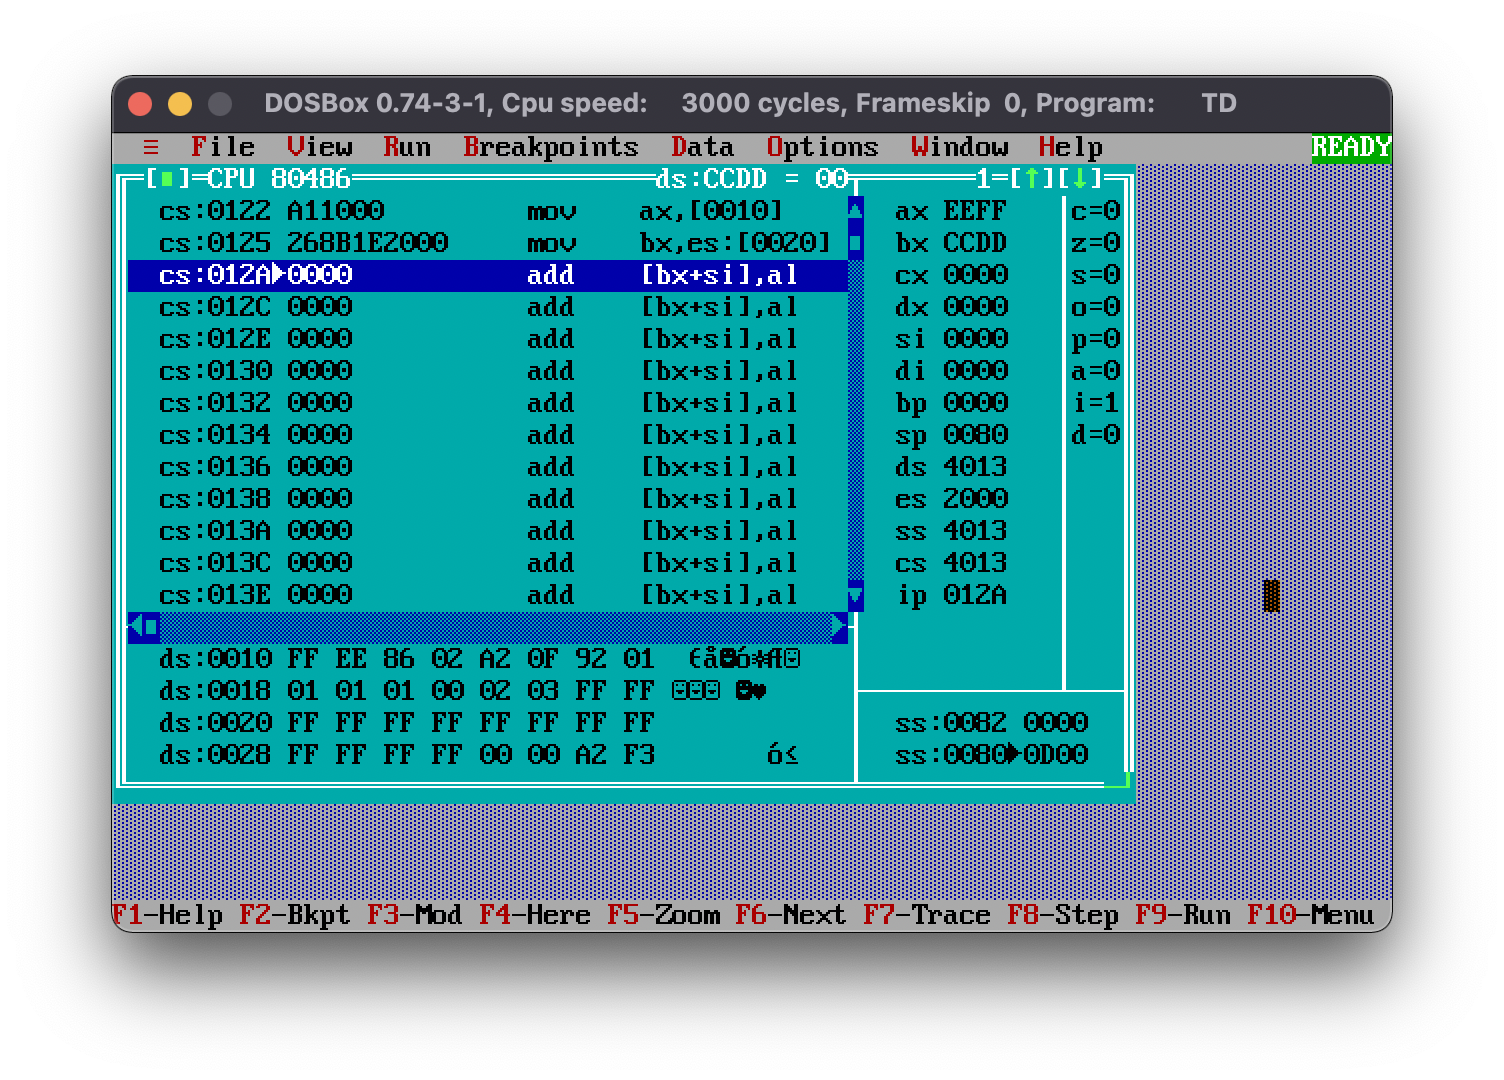
\includegraphics[width=0.7\textwidth]{fig/rlt7.png}
    \caption{}
    \label{fig:xxx}
\end{figure}

% 并排两张图样例
\begin{figure}[htbp]
    \centering
    \subfloat[原理图]{
        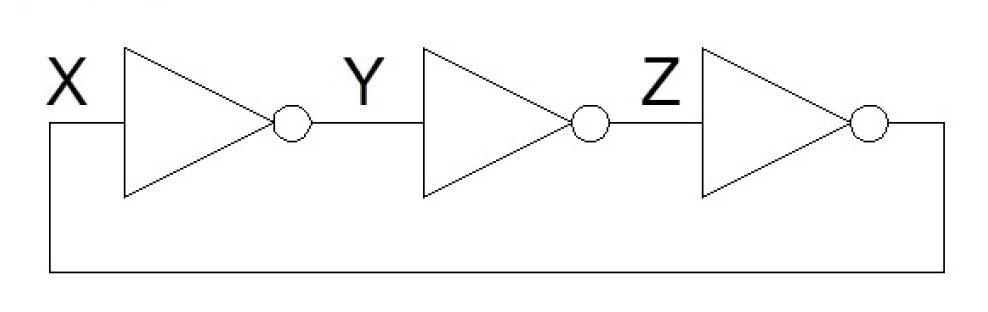
\includegraphics[height=2cm]{fig/oscillation_init.png}
        \label{subfig:oscillation_init}
    }
    \subfloat[等效图]{
        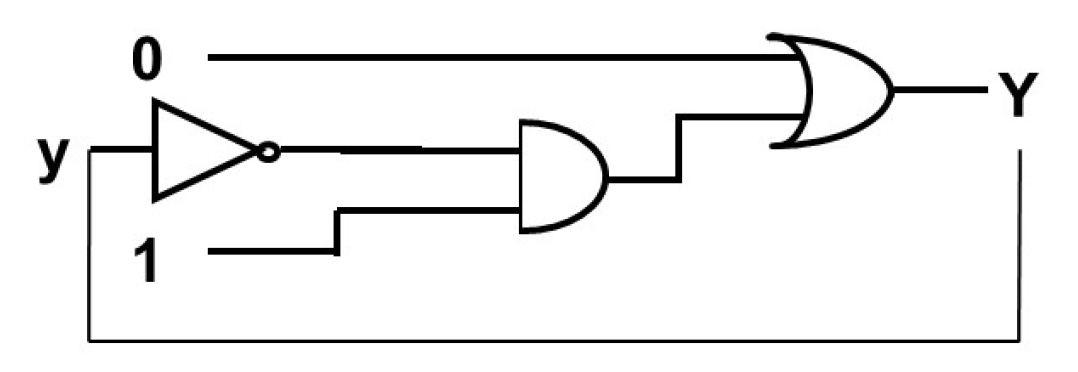
\includegraphics[height=2cm]{fig/oscillation_real.png}
        \label{subfig:oscillation_real}
    }
    \caption{}
    \label{fig:oscillation_circuit}
\end{figure}

% 注意样例(idea/analyze 分别表示思考和分析)
\begin{note}{题目}{}
    内容
\end{note}

% 代码样例
\begin{lstlisting}[language={[x86masm]Assembler},title=code]
    mycode
\end{lstlisting}